\documentclass[12pt]{article}

\usepackage{lads}

\setlength\parindent{0em}
\setlength\parskip{1em}

\title{FAQs: Support Vector Machines}
\date{}

\begin{document}

\maketitle

\textbf{Why do we use $\Va\cdot\Vx = b+1$ when training the SVM hyperplane but $\Va\cdot\Vx = b$ when classifying subsequent points?}

Let's use the SVM to classify two types of points, indicated as red and black circles below. The SVM algorithm pushes the parallel $\Va\cdot\Vx = b+1$ and $\Va\cdot\Vx = b-1$ hyperplanes outward until they hit the closest training points (the support vectors).

\begin{center}
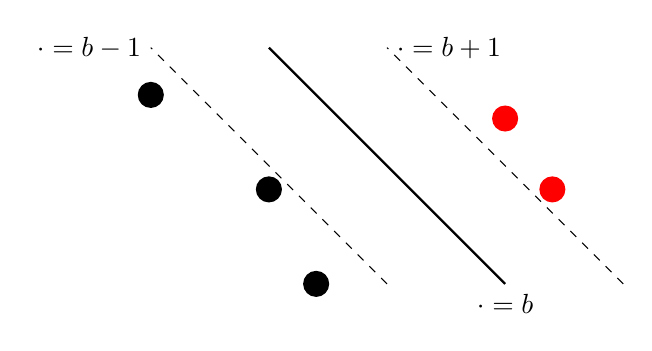
\begin{tikzpicture}[scale=3]
	\draw[thick] (0,1) -- (1,0) node[below] {$\Va\cdot\Vx=b$};
	\begin{scope}[xshift=0.5cm]
	\draw[dashed] (1,0) -- (0,1) node[right] {$\Va\cdot\Vx=b+1$};
	\end{scope}
	\begin{scope}[xshift=-0.5cm]
	\draw[dashed] (1,0) -- (0,1) node[left] {$\Va\cdot\Vx=b-1$};
	\end{scope}
	
	%\draw[style=help lines,step=0.2cm] (-2,-2) grid (2,2);
	
	\node at (0.0,0.4) [circle,fill=black] {};
	\node at (-0.5,0.8) [circle,fill=black] {};
	\node at (0.2,0) [circle,fill=black] {};
	
	\node at (1.2,0.4) [circle,fill=red] {};
	\node at (1.0,0.7) [circle,fill=red] {};
\end{tikzpicture}
\end{center}

Now that we've trained the SVM hyperplane, let's classify a new point. Imagine we want to classify the unknown (blue) point in the diagram below.

\begin{center}
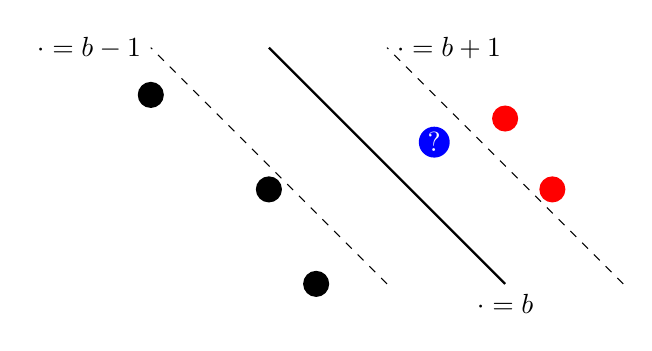
\begin{tikzpicture}[scale=3]
	\draw[thick] (0,1) -- (1,0) node[below] {$\Va\cdot\Vx=b$};
	\begin{scope}[xshift=0.5cm]
	\draw[dashed] (1,0) -- (0,1) node[right] {$\Va\cdot\Vx=b+1$};
	\end{scope}
	\begin{scope}[xshift=-0.5cm]
	\draw[dashed] (1,0) -- (0,1) node[left] {$\Va\cdot\Vx=b-1$};
	\end{scope}
	
	%\draw[style=help lines,step=0.2cm] (-2,-2) grid (2,2);
	
	\node at (0.0,0.4) [circle,fill=black] {};
	\node at (-0.5,0.8) [circle,fill=black] {};
	\node at (0.2,0) [circle,fill=black] {};
	
	\node at (1.2,0.4) [circle,fill=red] {};
	\node at (1.0,0.7) [circle,fill=red] {};
	
	\node at (0.7,0.6) [circle,fill=blue,inner sep=1pt,text=white] {?};
	
\end{tikzpicture}
\end{center}

It seems clear that the blue point should be classified with the red ones. However, it is below the $\Va\cdot\Vx = b+1$ hyperplane but still above the $\Va\cdot\Vx = b$ center hyperplane. We use the $\Va\cdot\Vx = b$ hyperplane for classification to handle points that are inside the outermost hyperplanes.
	
\end{document}
